\chapter{绪论}\label{chap:introduction}

\section{研究背景及意义}

分布式集群（如Hadoop、Kubernetes）是结合了分布式系统和集群系统优点的一种架构，在分布式集群中，不同的服务器负责不同的任务，同时每个任务可以由多个服务器组成的集群来处理。分布式集群是支撑现代云计算与大数据处理的核心基础设施，其稳定性直接关系到上层业务的连续性。此类集群在运行中会产生海量的多维度监控时序数据（如CPU负载、内存使用等），这些数据是感知系统健康状态、诊断异常的关键。

然而，随着集群规模不断扩大、架构动态性增强以及业务负载波动加剧，传统的基于阈值的异常检测方法因依赖先验知识、适应性差，导致误报和漏报率高，难以满足生产环境需求。尽管基于深度学习的方法能自动学习复杂模式，但在实际生产环境中，一个核心挑战在于对于如RPC连接数这类与用户任务相关的指标，其``正常''的绝对范围和模式难以统一定义，会随系统整体负载发生无规律波动，若使用基于历史数据训练的模型，会在整体高负载时产生大量误报，严重干扰运维效率。在分布式集群中，由于负载均衡机制的作用，在系统正常运行时，同一时刻各节点所承受的负载是相近的，各个节点指标曲线往往表现出极大的相似性，在运维实践中，运维人员常通过对比分布式集群中的同一指标曲线来判断异常：与其他变化模式相差很大的``离群曲线''更可能是异常。本研究正是基于这一洞察，旨在将``分布式集群相似性''这一先验知识系统性地引入多元时序异常检测模型，通过对比集群内多个节点在同一监控指标上的行为曲线，来识别其中显著偏离``群体一致性''模式的个别节点或子集，以提升异常检测的效果。

具体而言，本研究针对的是多节点时序数据集，即对同一指标（如CPU使用率）采集自集群中多个节点的、具有时间对齐关系的多条时序曲线。该数据集不仅包含每个节点自身的时序变化模式，更隐含了节点之间的运行关联与协同规律。如何有效捕捉并利用这种分布式关联，构建能够区分节点个体异常与集群整体波动的检测模型，是本研究要解决的关键问题。

本研究的意义在于，从方法和实践应用两个层面为分布式集群异常检测提供了新的思路与解决方案。在方法层面，本研究跳出了传统异常检测聚焦于``时间''与``指标''二维分析的框架，创新性地将``集群节点''这一空间维度系统性地引入模型，构建了``时间$\times$指标$\times$节点''的三维分析范式。这一范式将集群内在的、由负载均衡机制保证的节点行为相似性，从一种隐性的运维经验转化为一种显式的、可计算的先验知识，为处理动态负载场景下的异常检测问题提供了新的视角。在实践应用层面，所提出的方法直接针对生产环境中负载敏感型指标检测的痛点，通过识别``离群曲线''而非定义``绝对正常''，能够有效降低因集群整体负载波动引发的误报，提升检测结果的可靠性。基于真实运维数据构建数据集并验证算法，既保证了方法在实际业务场景下的有效性，也为后续研究提供了数据基础。本研究结果不仅有助于实现更精准的故障定位与预警，缩短平均故障恢复时间，提升业务连续性，也为提升真实集群运维体系智能化提供了核心的检测能力支撑，具有重要的工程应用价值。

\section{国内外研究现状}

时间序列异常检测是数据挖掘和机器学习领域的重要研究方向，旨在识别时间序列数据中偏离正常行为模式的异常点或异常序列。随着物联网、工业4.0和金融科技的发展，时间序列数据规模呈指数级增长，对高效、准确的异常检测方法提出了更高要求。纵观该领域的发展历程，研究方法呈现出清晰的演进脉络：从基于严格统计假设的传统方法，到依赖特征工程的经典机器学习方法，再到能够端到端自动学习复杂模式的深度学习方法，体现了从模型驱动向数据驱动的智能学习范式转变。

传统统计方法奠定了异常检测的理论基石，其核心思想是基于概率分布假设进行统计推断，将显著偏离统计特性的观测点判定为异常。最具代表性的是3-sigma准则，该方法假设数据服从正态分布，根据切比雪夫不等式的推论，正常数据落在均值$\mu$加减三倍标准差$\sigma$区间内的概率约为99.7\%，因此将落在该区间之外的点视为异常。然而，该方法对分布假设敏感，且难以处理存在多个离群值的情况。针对单个离群值的检测，Grubbs检验\cite{grubbs1969}提供了更严谨的统计框架，其检验统计量定义为$G = \frac{\max|x_i - \bar{x}|}{s}$，通过与基于样本量和显著性水平确定的临界值比较来判断异常，该方法适用于样本量较小且仅含单个离群值的场景。Dixon检验\cite{dixon1950}（又称Q检验）则通过计算可疑值与相邻值的差异相对于数据全距的比例来判断异常，其计算简便且对极端值检测具有较好的鲁棒性。对于多变量场景，上述单变量方法存在明显局限，因为异常点可能在各单变量上并不极端，但其变量组合模式偏离正常关联结构。Mahalanobis距离\cite{mahalanobis1936}通过引入协方差矩阵来度量样本点偏离分布中心的程度，其定义为$D_M = \sqrt{(\mathbf{x}-\boldsymbol{\mu})^T \boldsymbol{\Sigma}^{-1} (\mathbf{x}-\boldsymbol{\mu})}$，能够有效识别这类多变量关联异常。此外，基于时序模型的方法如ARIMA\cite{box1970arima}通过差分运算将非平稳序列转化为平稳序列，再结合自回归和移动平均成分建模时间序列的自相关结构，将预测残差作为异常判据；分解方法如STL\cite{cleveland1990stl}采用局部加权回归将时间序列分解为趋势、季节和残差三个成分，通过分析残差成分中的极端值来识别异常。传统统计方法原理简单、可解释性强，但严重依赖分布假设，在面对复杂非线性模式和高维数据时能力有限。

经典机器学习方法拓展了异常检测的实用边界，其核心转变是从基于分布假设转向基于数据特征的相似性或密度度量。距离基方法直接利用距离度量分析样本间的相似性，其基本假设是异常点与正常点之间的距离较大。K近邻方法\cite{ramaswamy2000}通过计算每个样本到其第K个最近邻居的距离作为异常分数，距离越大则越可能是异常。密度基方法则从局部密度的角度刻画异常，其中局部离群因子（LOF）\cite{breunig2000lof}是最具代表性的算法，它通过比较样本点的局部可达密度与其邻居的局部可达密度来计算离群因子，LOF值显著大于1表明该点相对于其邻域更加稀疏，因而更可能是异常。与距离基方法相比，LOF能够更好地处理密度分布不均匀的数据。隔离基方法以孤立森林\cite{liu2008isolation}为代表，其核心思想源于一个直观的观察：异常点由于``少且不同''的特性，在随机分割构成的树结构中更容易被隔离出来。具体而言，算法通过随机选择特征和分割点递归划分数据空间构建隔离树，异常点由于偏离正常数据密集区域，通常只需较少的分割次数即可被隔离，因此其在树中的平均路径长度较短。孤立森林的时间复杂度为$O(n\log n)$，相比需要计算成对距离的方法具有显著的效率优势，因此在工业界得到广泛应用。这些经典方法的共同优势在于无需大量标注数据，但效果依赖于精心设计的特征工程，且由于未显式建模时间依赖关系，难以有效捕捉时间序列中复杂的非线性关系和长期依赖。

深度学习方法实现了异常检测性能的显著突破\cite{choi2021deepreview,pang2021deepsurvey}，其核心创新是利用神经网络自动学习数据的内在表示，摆脱了对人工特征工程的依赖。重构型方法以自编码器及其变体为代表，其核心假设是：模型在正常数据上训练后学习到了正常模式的低维表示，当输入异常数据时由于其模式未被学习，解码器难以准确重构，从而产生较大的重构误差。OmniAnomaly\cite{su2019omni}在此基础上引入随机变分推断和归一化流，通过建模正常数据的复杂潜在分布来提升检测能力；USAD\cite{audibert2020usad}则采用两个共享编码器的解码器进行对抗训练，增强了模型对异常的敏感性。预测型方法利用序列模型的时序建模能力，通过预测未来时间步的取值并将预测误差作为异常分数。长短期记忆网络（LSTM）\cite{hochreiter1997lstm}通过门控机制有效缓解了梯度消失问题，能够捕捉序列中的长期依赖关系。近年来，Transformer架构凭借其强大的自注意力机制在时序建模中展现出优势，TranAD\cite{tuli2022tranad}采用两阶段对抗训练机制，通过``自调节''策略放大异常样本的重建误差；Anomaly Transformer\cite{xu2022anomaly}则提出关联差异性概念，利用异常点在时序关联模式上的特殊性进行检测。在多变量时序场景中，如何建模变量间的复杂依赖关系是核心挑战。图神经网络因能够显式建模变量间的拓扑关系而被广泛应用，GDN\cite{deng2021graph}通过注意力机制自动学习传感器之间的图结构，并基于图卷积网络进行预测。此外，基于因果分析的方法将异常视为偏离正常因果机制的实例，CAROTS\cite{chen2025carots}创新性地将因果关系融入对比学习框架，通过设计保持因果结构和破坏因果结构的两类数据增强策略，训练模型在潜在空间中区分正常与异常样本，同时支持异常根因定位。深度学习方法的主要优势在于强大的表征学习能力，但也面临训练不稳定、计算资源需求高、可解释性差等局限。

在研究趋势方面，当前领域呈现出多个重要发展方向。频域分析与时域分析的结合成为提升检测能力的新途径\cite{ren2019sranomaly}，通过傅里叶变换等方法从频率视角捕捉异常模式。对比学习与自监督学习的兴起为解决标签稀缺问题提供了新思路\cite{darban2025carla}，通过设计有效的数据增强策略从无标签数据中学习鲁棒表征。可解释性与评估标准化受到越来越多的重视，因果推断方法被引入以增强模型透明度，专门化评估指标如VUS-PR\cite{paparrizos2022tsbuad}和综合性基准框架如TAB\cite{wu2024tab}不断涌现，为公平比较不同方法提供了平台。随着数据规模的增长，分布式系统架构的发展也成为必然趋势，基于Spark\cite{fan2015spark}、Flink\cite{carbone2015flink}等框架的系统实现了大规模时序数据的高效处理。

总体来看，现有研究虽然取得了显著进展，但绝大多数工作仍聚焦于时间与指标这两个维度构成的二维数据分析框架内。一个普遍的局限性在于，未能系统性地挖掘和利用分布式集群生产环境中广泛存在的多节点这一宝贵维度信息，忽视了同一集群内各节点指标行为模式的内在相似性及其对异常判别的辅助价值。因此，本研究旨在填补这一空白，探索一种基于时间、指标与集群节点的三维数据分析新范式，以期提升异常检测在真实动态运维场景中的鲁棒性。

\section{论文研究内容和贡献}

\subsection{主要研究内容}

本文围绕分布式集群多节点场景下的时序异常检测问题，开展了以下三个方面的研究工作。

第一，面向单指标多节点场景的异常检测算法研究。本文以YARN集群的RPC Router连接数指标为研究对象，构建了基于联通大数据生产环境的单指标多节点时序数据集。在此基础上，分别采用欧氏距离、自编码器嵌入距离和密度偏离三种方法度量节点曲线间的相似性，验证了基于群体一致性思想的异常检测方法的有效性。针对单一方法阈值高度敏感的问题，提出了I-SPOT（Inclusive SPOT）包容性自适应阈值算法，通过将所有数据点纳入模型更新池解决经典SPOT在概念漂移场景下的阈值衰减问题。在此基础上，将多视角相似性评分、分数归一化聚合与I-SPOT自适应阈值检测整合为统一的CSAD-AT框架，实现端到端的自适应异常检测。

第二，面向多指标多节点场景的异常检测算法研究。本文使用真实GPU集群故障数据集，针对多指标场景下数据规模增长带来的算法效率约束以及异常表现异质性导致的检测盲区问题，设计了NSFusion数值与形状双视角融合的异常检测框架。该框架放弃了单指标场景中计算开销较大的自编码器和密度偏离方法，在数值视角方面采用优化的基于欧氏距离的多指标加权融合方法量化节点间的数值差异，在形状视角方面提出FR-SAX（Full-Resolution SAX）符号化表示算法作为自编码器的轻量化替代方案，通过取消分段聚合保留原始分辨率并采用严格距离计算规则来捕捉曲线形态差异。最终通过加权融合两种视角的检测结果，实现对不同类型异常的全面覆盖。

第三，基于曲线相似性的异常检测系统设计与实现。本文设计了面向分布式集群的异常检测系统，采用前后端分离的四层架构，实现了从数据采集、预处理、异常检测到结果展示的完整流程。系统支持文件上传和Prometheus API两种数据接入方式，通过APScheduler定时任务框架实现对多个集群的常态化自动巡检，并构建了三级告警机制支持邮件和企业微信等多渠道通知。系统已具备对接联通大数据生产底座平台Prometheus监控体系的接口能力，并通过历史数据回放验证了功能完整性。

\subsection{主要贡献}

本文的主要贡献包括以下三个方面。

第一，本文提出了一种基于多节点曲线相似性的分布式集群异常检测方法。该方法突破了传统异常检测聚焦于时间与指标二维分析的框架，创新性地将集群节点这一空间维度系统性地引入模型，构建了时间、指标与节点的三维分析范式。通过利用分布式集群负载均衡机制所保证的节点行为相似性，将隐性的运维经验转化为显式的可计算先验知识。

第二，本文设计了兼顾计算效率与检测覆盖面的数值与形状双视角融合多指标异常检测框架。针对多指标场景下数据规模成倍增长的效率约束，框架采用轻量化的数值距离计算与无需训练的符号化形状度量相结合的方案；针对不同指标间异常表现异质性导致的单一视角检测盲区，框架从数值幅度和曲线形态两个互补角度刻画节点异常行为，其中FR-SAX（Full-Resolution SAX）算法通过保留原始分辨率和采用严格距离计算规则增强了对形状变化的敏感性。通过加权融合两种视角的检测结果，该框架能够有效识别不同类型的节点异常。

第三，本文基于联通大数据真实生产环境构建了单指标多节点时序数据集，并使用阶跃星辰GPU集群故障数据集进行多指标多节点场景的验证。在这些数据集上的实验结果表明，本文所提方法在检测准确率方面显著优于现有的多元时序异常检测算法。此外，本文设计并实现了完整的异常检测系统，支持常态化自动巡检和多级告警，具备对接实际生产环境的接口能力，为分布式集群异常检测提供了从算法到系统的完整解决方案。

\section{论文组织结构}

本文共分为六章，各章内容安排如下。

第一章绪论部分阐述了本研究的背景与意义，回顾了多元时间序列异常检测领域的国内外研究现状，概述了本文的主要研究内容与贡献。

第二章介绍了相关背景知识与理论基础，包括时间序列异常的定义与分类、主流的时序异常检测算法，以及分布式集群监控数据的特点与挑战。各章实验所采用的评估指标在对应的实验设置部分进行介绍。

第三章针对单指标多节点场景，详细介绍了数据集的构建过程、基于曲线相似性的三种异常检测方法和参数敏感性分析，以及I-SPOT包容性自适应阈值算法和CSAD-AT框架的设计。

第四章针对多指标多节点场景，以阶跃星辰GPU集群故障数据集为基础，提出了数值与形状双视角融合的异常检测框架，详细阐述了基于欧氏距离的数值异常检测算法和基于FR-SAX的形状异常检测算法，并介绍了多算法融合与故障定位方法。

第五章介绍了基于曲线相似性的异常检测系统，包括系统的总体流程设计、架构与关键技术、实现细节及应用效果展示。

第六章对全文工作进行总结，并对未来研究方向进行展望。

本文的研究内容框架如图\ref{fig:research_framework}所示。

\begin{figure}[H]
    \centering
    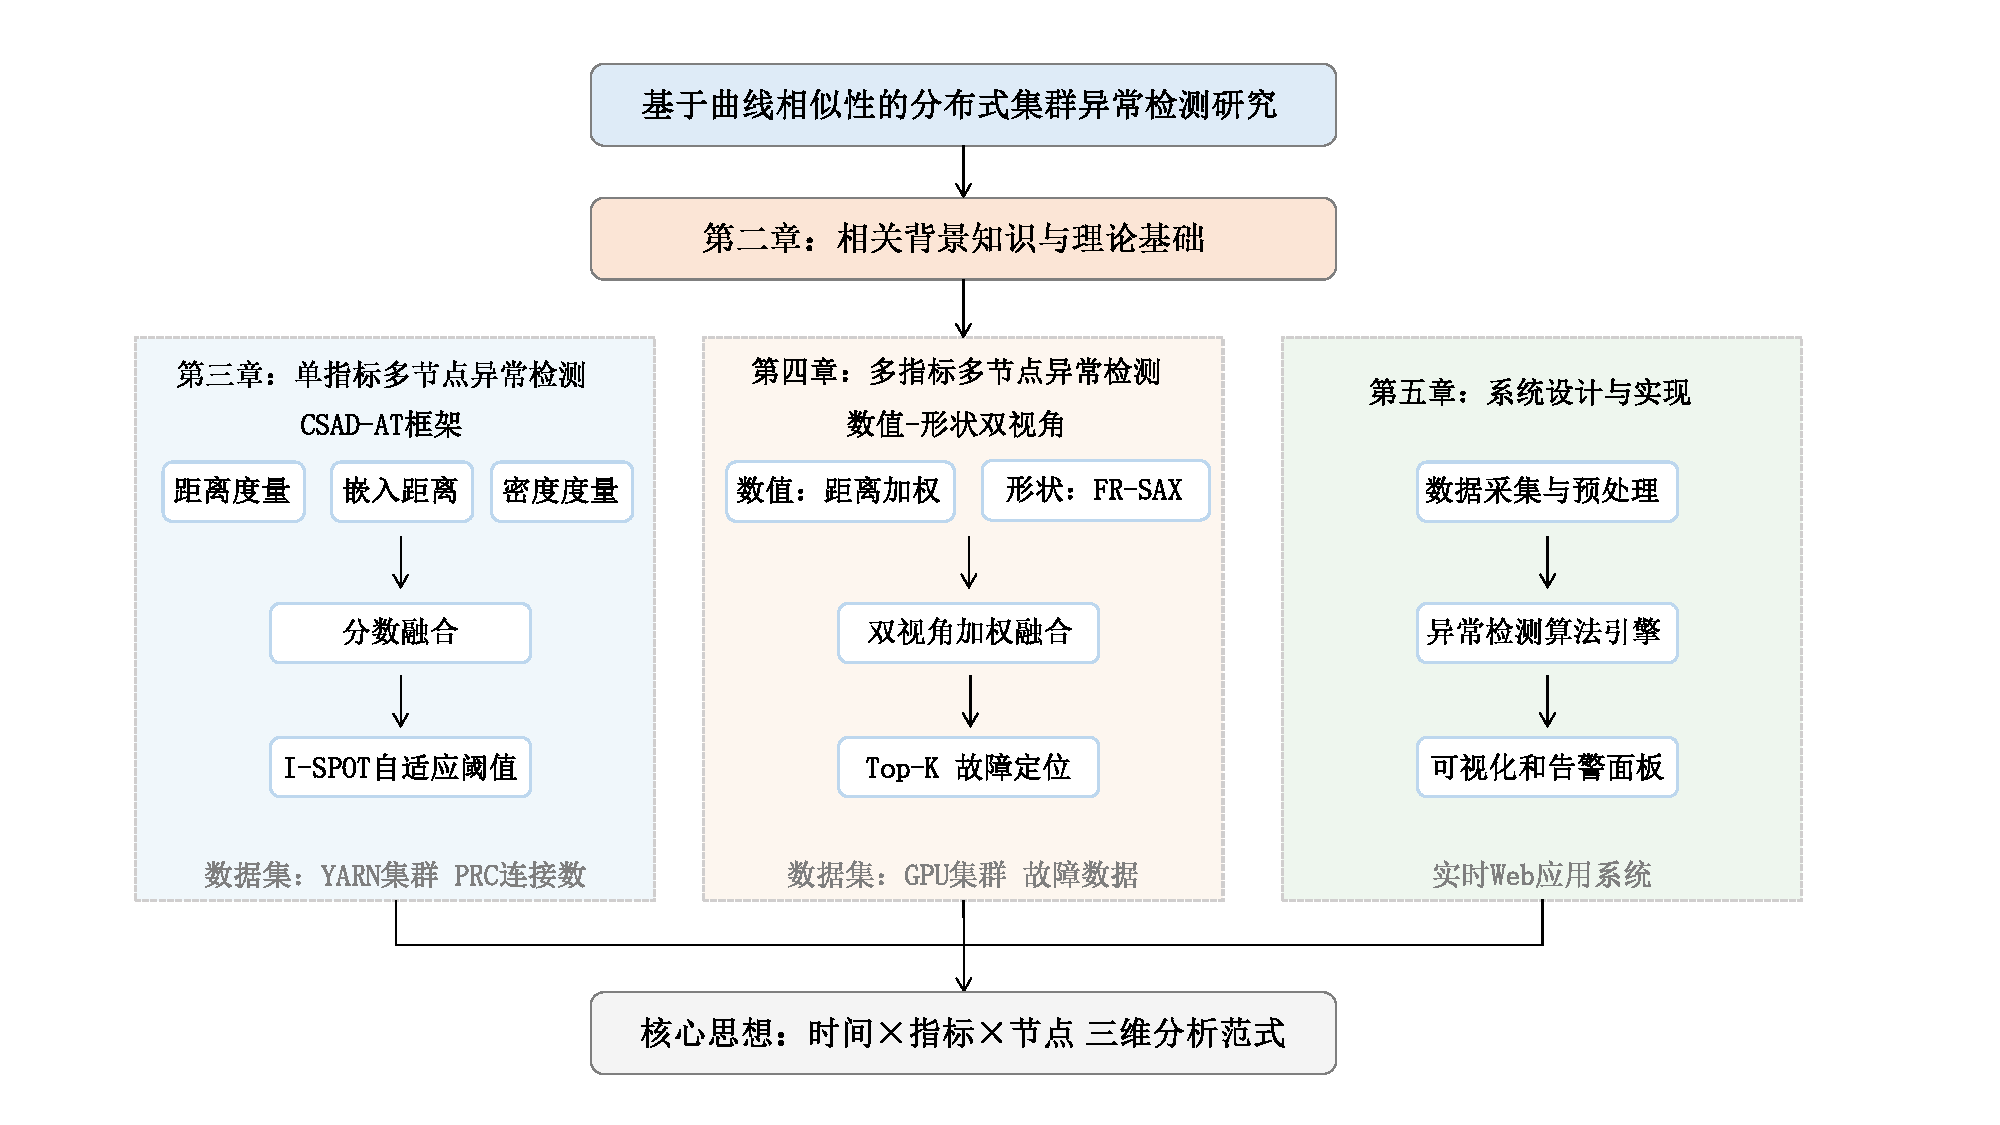
\includegraphics[width=\textwidth]{Img/research_framework.pdf}
    \bicaption{\enspace 论文研究内容框架图}{\enspace Research Content Framework of This Thesis}
    \label{fig:research_framework}
\end{figure}
